% !TEX program = xelatex

\documentclass[12pt,a4paper]{article}

\usepackage{amsthm,amsfonts,amssymb,bm}
\usepackage[fleqn]{amsmath}

% Page settings
\addtolength{\textheight}{2.0cm}
\addtolength{\voffset}{-2cm}
\addtolength{\hoffset}{-1.5cm}
\addtolength{\textwidth}{4.0cm}

%\allowdisplaybreaks

%\usepackage{subeqnarray}
\usepackage{mathrsfs}
%\usepackage{color}
%\usepackage{url}
%\usepackage{ulem}
\usepackage{indentfirst}   % Indent first line of a paragraph
%\usepackage{textcomp}




%%Here is the configuration for chinese. setmainfont is the default font of the text.
\usepackage[cm-default]{fontspec}
\usepackage{xunicode}
%\usepackage{xltxtra}
\setmainfont{"微软雅黑"}
%\setmainfont{AR PL UKai CN}
%\setsansfont[BoldFont=SimHei]{KaiTi_GB2312}
%\setmonofont{NSimSun}



\XeTeXlinebreaklocale "zh"
%\XeTeXlinebreakskip = 0pt plus 1pt

% Figure, Diagram, Caption settings
%\usepackage{tikz}
%\usetikzlibrary{mindmap,trees}
\usepackage{graphicx}
%\usepackage{graphics}
%\usepackage[hang,small,bf]{caption}
%\setlength{\captionmargin}{50pt}

% Redefine some fonts.
%\newfontfamily\heiti{"黑体"}
%\newfontfamily\fs{"仿宋"}
%\newfontfamily\yahei{"微软雅黑"}


\graphicspath{{Figure/}}

\begin{document}
\title{\Huge 中文XeLaTeX}


\author{XXXXX}
%\maketitle

% Redefine some math commands and environments.

\newcommand{\dd}{\mathrm d}
%\newcommand{\HH}{\mathcal H}
%\newcommand{\CN}{{\it Cosmologia Notebook}}
\newenvironment{eqnset}
{\begin{equation}\left \bracevert \begin{array}{l}}
{\end{array} \right. \end{equation}}

\newenvironment{eqn}
{\begin{equation}\left \bracevert \begin{array}{l}}
{\end{array} \right. \end{equation}}





因为是球对称的球体,所以其线元应该是Schwarzschild的

\begin{equation}
\mathrm ds^2 = -(1-\frac{2m(r)}{r})c^2 \mathrm dt^2 + (1- \frac{2m}{r})^{-1}\mathrm d r^2 +r^2 (\mathrm d\theta^2 + \sin^2\theta \mathrm d\phi^2)
\end{equation}

使用与时间轴正交的超曲面,直接取后面的空间部分。这样一个实际上这个球体的物理的体积应该是

\begin{eqnarray}
V(R,M)&=&\int \frac{1}{\sqrt{1-\frac{2m(r,M,R)}{r}}} r^2 \sin\theta \mathrm dr\mathrm d\theta\mathrm d\phi \\
&=&4\pi^2 \int \frac{1}{\sqrt{1-\frac{2m(r)}{r}}}r^2 \mathrm dr
\end{eqnarray}
其中$m(r,M)$是质量分布函数,$M$是球体总质量,$R$是球体的半径,这个半径是指的在Schwarzschild度规中的坐标值。

用一个特殊的均匀分布
\begin{equation}
m(r)=\frac{4/3 \pi r^3}{4/3 \pi R^3}=(\frac{r}{R})^3 M
\end{equation}

可以对体积积分进行简化
\begin{equation}
V=4\pi^2 \int \frac{1}{\sqrt{1-2 M \frac{r^2}{R^3}}}r^2\mathrm dr
\end{equation}

最后球体的密度可以通过$\rho=M/V$来计算。

密度随R或者M变的曲线可以绘制出了。


下图是球体的半径$R$一定的时候,密度随着质量$M$的变化曲线。
\begin{figure}[!htbp]
\centering
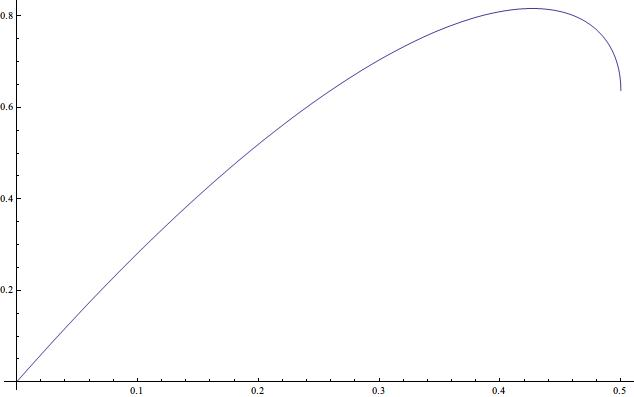
\includegraphics[width=400pt]{DustBlackHole_FixR.jpg}
\caption{球体半径为1,密度随质量的变化。}\label{fig:FixR}
\end{figure}

现在可以看到,随着质量增加,密度先是增加,后来减小,有一个峰值。也就是说,如果现在有个区域半径为1,我们不停的往里面添加尘埃,并且使其分布满足上面提到的特定的均匀质量分布,这样这个尘埃团的密度先增加,直到质量达到0.427的时候,密度达到最大值0.816,之后密度反而开始减小,最后直到形成黑洞前,密度减小到$2/\pi$。图中可以看到,在$M=0.5$的地方,斜率可能是负无穷。经过计算得知,这个猜想是正确的。也就是说,如果趋势不变,在$M=0.5$这个点,球体的密度将垂直降到0!很奇怪。

进一步想,密度降下来,按照古旧的观点来看,只能是体积减小了,因为我们一直往其中添加物质。从体积的表达式中也可以看出来。那么形成黑洞的时候,体积确实变成了无穷大?

这点有点奇怪。如果体积变成了无穷大,那么很多定律都变得不合理。我们是否可以把部分效应转移到质量上去而使得体积不出现奇性么?甚至体积变为零最好了。因为这样就可以跟Hollowgraphic吻合起来了。

密度的表达式写完整应该是这样的:
\begin{eqnarray}
\rho(M,R)&=&\frac{-2 R\sqrt{M(-2M R^2+R^3)}+\sqrt 2 R^3 \arcsin (\sqrt{2 \frac{M}{R}})}{8 (\frac{M}{R})^{3/2}}\label{eqn:densityMR}
\end{eqnarray}

这里面的\(M\)是引力质量,因为这个质量要用来对时空的度规产生影响,从而顺便改变体积积分。这个是很麻烦的,因为改动之后还有保持质量、密度和体积的表达式的自洽性。
如果引力理论不是像Einstein那样使用等效原理,而是对质量这个概念作了手脚,比如引力质量换成场的耦合系数之类,就可以实现引力质量随着引力场强增加而减小的效果。具体如何实现,可以拿Scalar Tensor理论来看看。
不过改动强引力场的部分会对宇宙学造成比较大的影响,因为一般要求早期宇宙的引力理论不要与Einstein的差别太大,至少造成的可观测效果不要有太大偏离。

下图是球体的质量$M$一定的时候,密度随着半径$R$的变化曲线。
\begin{figure}[!htbp]
\centering
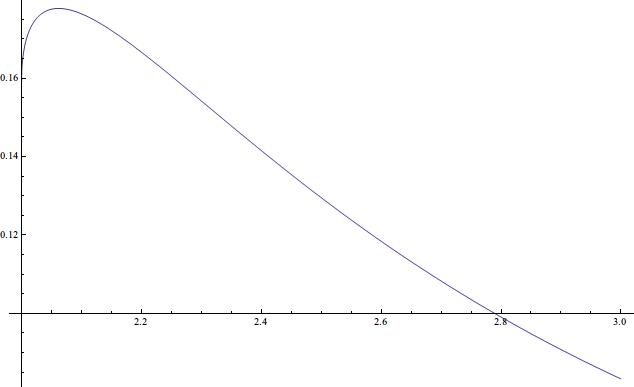
\includegraphics[width=400pt]{DustBlackHole_FixM.jpg}
\caption{球体质量为1,密度随半径的变化。}\label{fig:3D}
\end{figure}

用来补足上面的分析。现有一个质量为1的尘埃球,当$R$从3开始越来越小的时候,密度先变大后变小。峰值出现在$R=2.062$的地方,最大密度为$\rho=0.178$。当$R=2$时,密度为$\rho=2/\pi$。如果半径小于2,就会成为黑洞了。与上面的讨论质量的情况吻合。


当然,如果想比较完整的了解一下这个函数的特性,可以做出3D视图
\begin{figure}[!htbp]
\centering
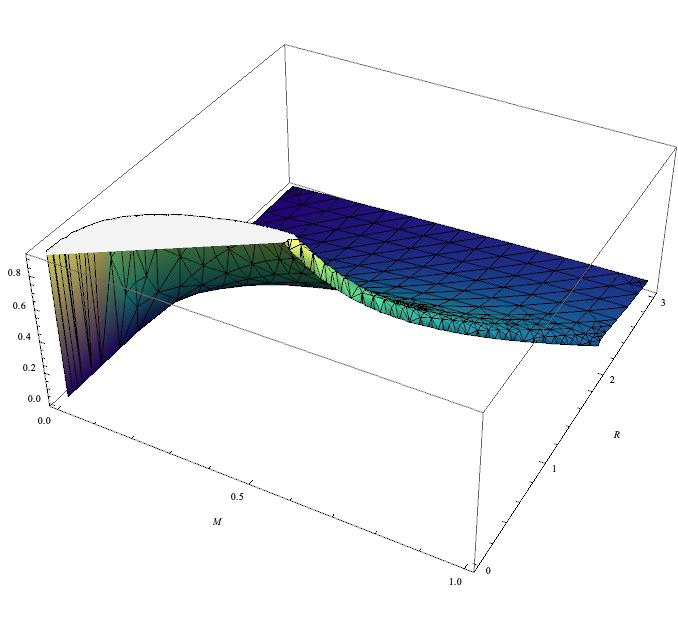
\includegraphics[width=400pt]{DustBlackHole_3D.jpg}
\caption{球体密度随质量和半径的变化。}\label{fig:FixM}
\end{figure}


\vspace{3em}


\bf 最后,其实还有个值得思考的问题,上面这个讨论对于不同的质量分布,是不是都适合的?比如换另一种均匀质量分布的表达式?

\end{document}